% ─────────────────────────────────────────────────────────────────────────────
\chapter{GUI Workflow and Example}
\label{sec:gui}
% ─────────────────────────────────────────────────────────────────────────────

Launch the GUI from the terminal:

\begin{lstlisting}[language=bash]
sundic
\end{lstlisting}

The GUI presents a five-tab workflow (Figure~\ref{fig:gui_settings}), where each tab must be completed in order before proceeding to the next. Hovering over any input field displays a tooltip explaining the corresponding parameter.

The sections below describe each menu item and tab, followed by instructions for running the included example problem.

\section{File Menu}

The \codebf{File} menu provides session management functionality as follows:

\begin{itemize}
	\item \codebf{New} -- Clear all settings and start a new session.
	\item \codebf{Open} -- Load a previously saved \code{.sdic} file. This is a binary file that may contain settings and/or results. It is generated either by the GUI or the API, in which case it can be opened for post-processing in the GUI.
	\item \codebf{Import Settings File} -- Populate all GUI fields from an existing \code{settings.ini} file.
	\item \codebf{Export Settings File} -- Save the current GUI settings to a \code{settings.ini} file for use with the API.
	\item \codebf{Save} / \textbf{Save As} -- Save the current session under a specified name. This will create a \code{.sdic} binary file.
	\item \codebf{Exit} -- Close the application.
\end{itemize}

Importing and exporting configuration files is the fastest way to share or reuse configurations. The exported file is identical to the INI format described in Section~\ref{sec:parameters}.

\section{Settings Tab}

The \codebf{Settings} tab is used to configure all global DIC parameters before loading images and defining the ROI. The fields are arranged in two columns and correspond directly to the parameters defined in Section~\ref{sec:parameters}.

The \codebf{Set Defaults (For this Panel Only)} button may be used to restore factory defaults for this tab only without affecting other settings.

\begin{figure}[!hbtp]
	\centering
	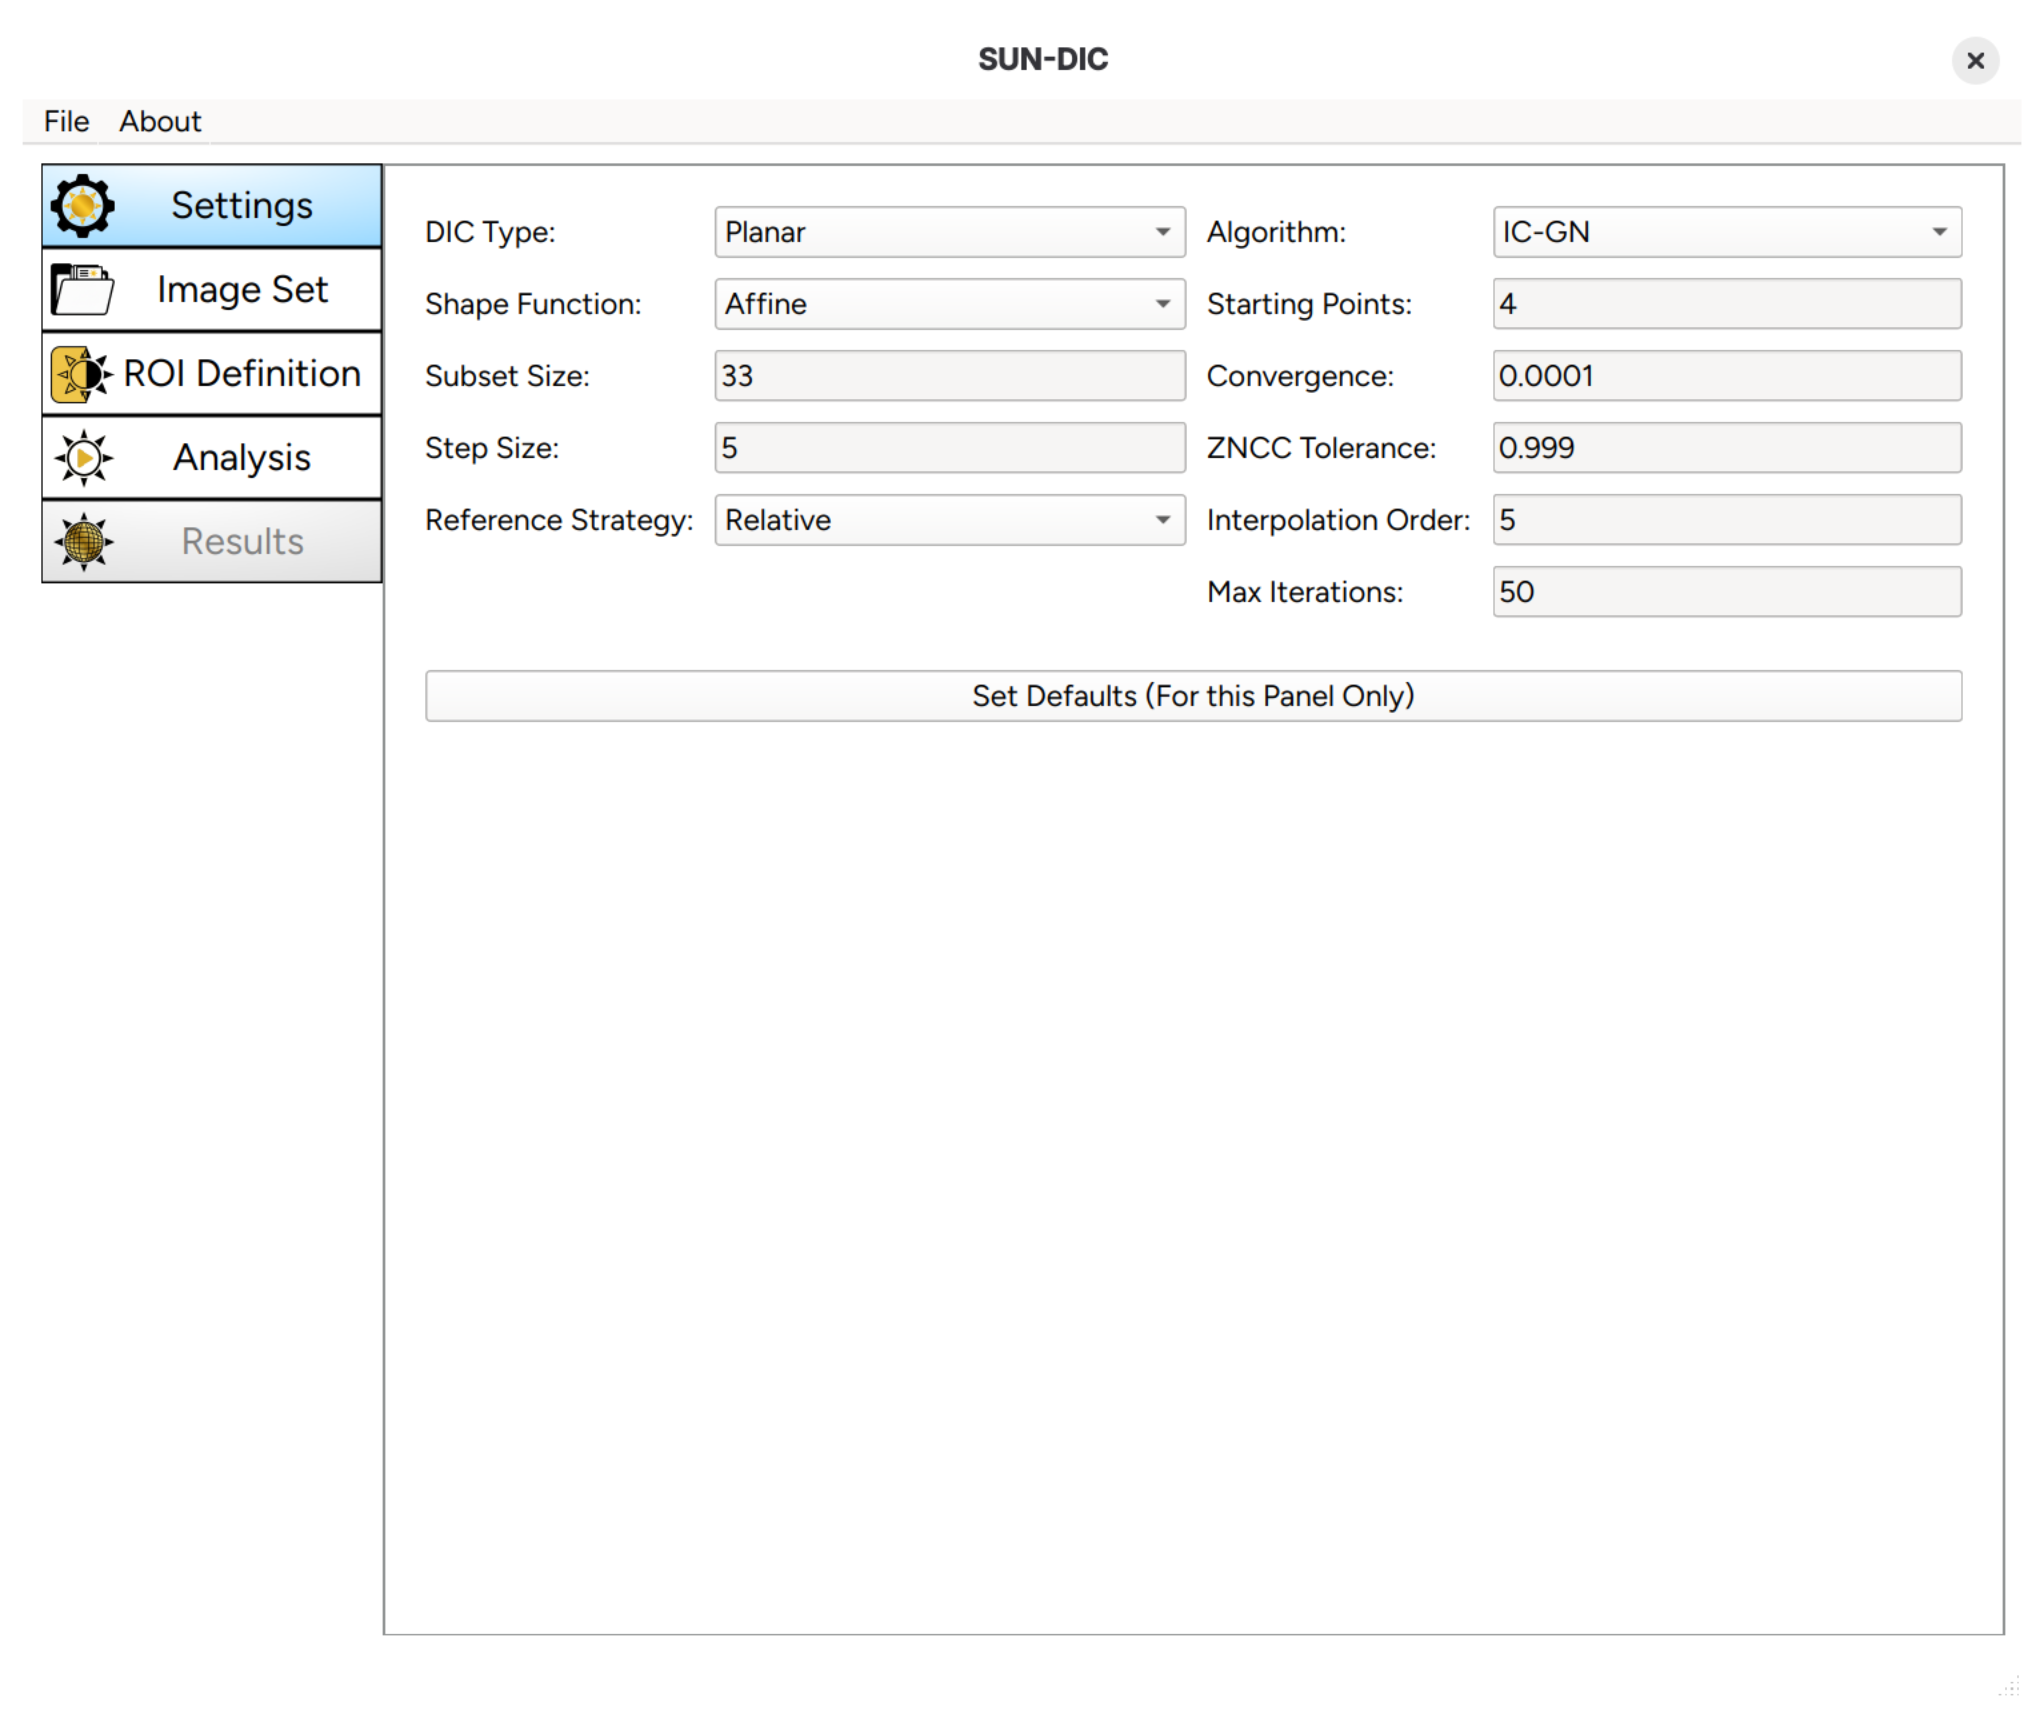
\includegraphics[width=0.85\textwidth]{../../screenshots/settings.png}
	\caption{Settings Tab. General SUN-DIC parameters are configured here.}
	\label{fig:gui_settings}
\end{figure}

\section{Image Set Tab}

The \codebf{Image Set} tab is used to define the image set that will be used during the DIC analysis. Click the \codebf{Select Directory} button to choose the folder containing the image sequence. This folder should contain only the image sequence, as all files in the directory will be considered. The selected folder path is displayed in the \codebf{Folder} field. Images are considered in natural sort order.

To define the image set, the first and last images in the range are specified using the \codebf{Start} and \codebf{End} fields, while the \codebf{Increment} field defines the spacing between images in the sequence. The \codebf{Set Max} button can be used to automatically set the \codebf{End} field to the last image in the folder. The default behaviour is to consider all images in the selected image folder. The selected images are displayed in the \codebf{Images} list.

The \textbf{Advanced Settings} area exposes two pre-processing parameters: Gaussian blur kernel size (for noise reduction) and the background cut-off value. The background cut-off is used to automatically detect dark regions (e.g.\ holes) that are treated as background and automatically excluded from the ROI. Subsets with mean intensity below the specified threshold value are ignored.

The \textbf{Set Defaults (For this Panel Only)} button may be used to restore factory defaults for this tab only without affecting other settings.

\begin{figure}[!hbtp]
	\centering
	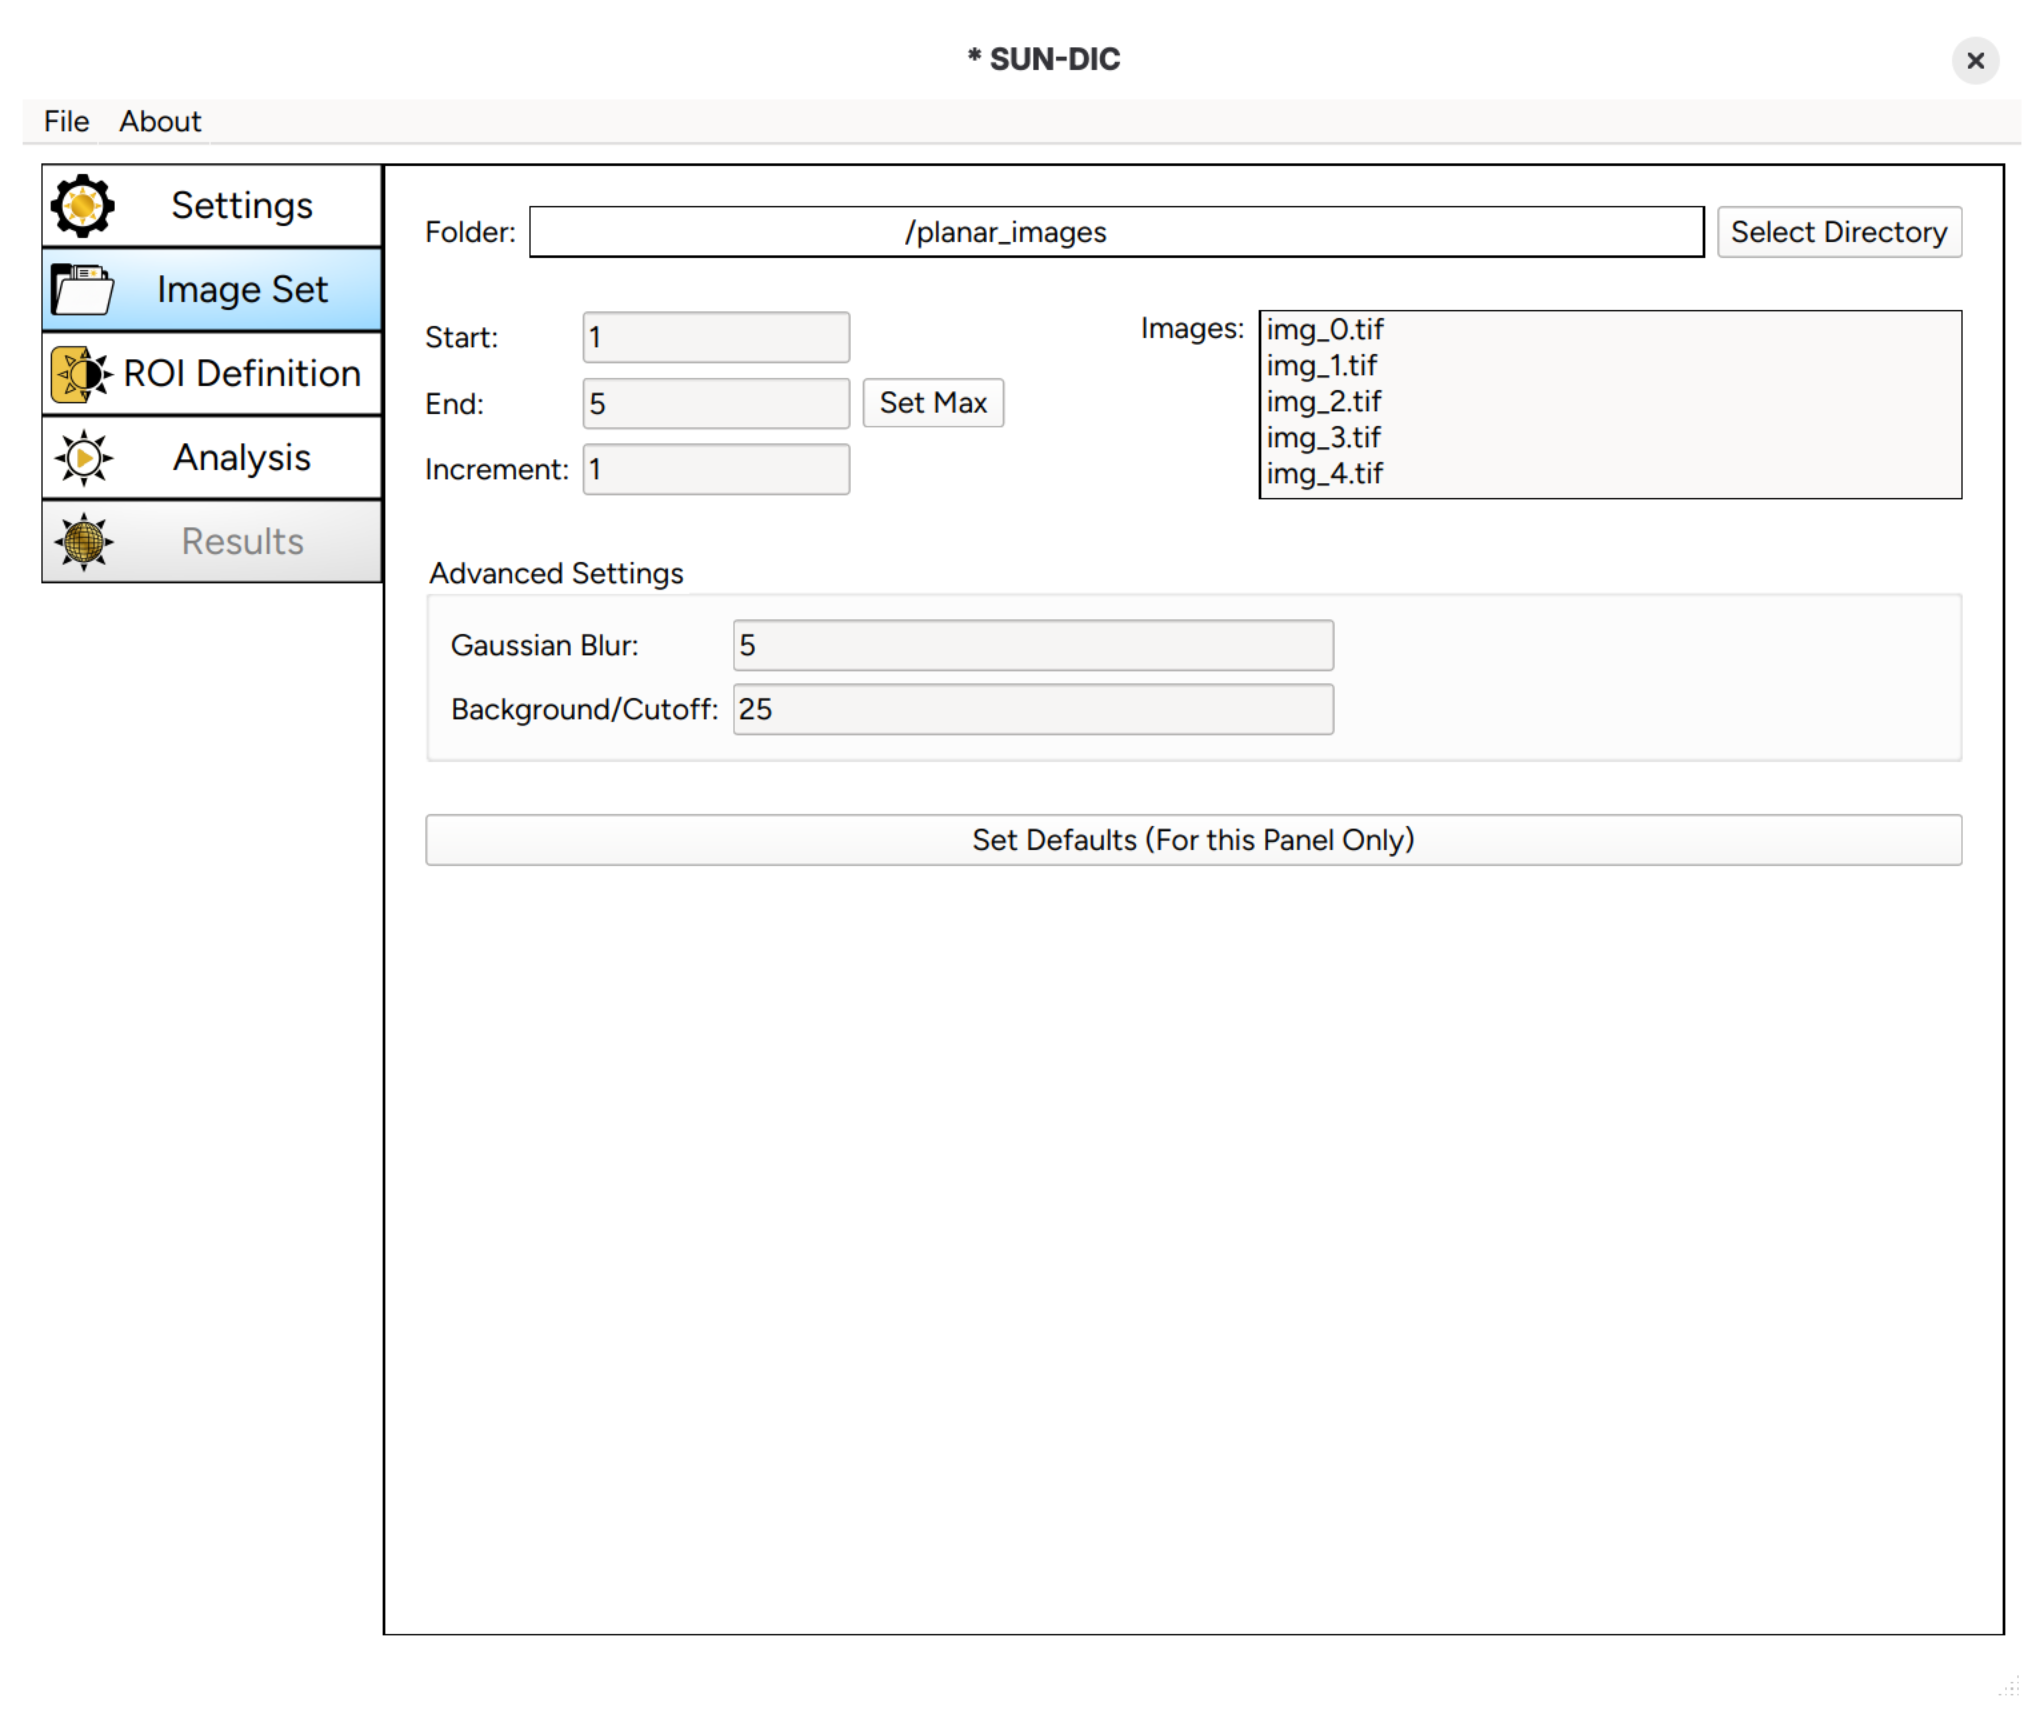
\includegraphics[width=0.85\textwidth]{../../screenshots/image_set.png}
	\caption{Image Set Tab. Select image folder, datum image, and target range.}
	\label{fig:gui_imageset}
\end{figure}

\section{ROI Definition Tab}

The \codebf{ROI Definition} tab is used to define and visualise the ROI. The datum image selected in the \codebf{Image Set} tab is displayed in an interactive viewer where the ROI is defined. The ROI is defined by clicking and dragging the mouse over the image to draw a rectangular region. It is shown as a red outline, and green markers indicate active subset centres so that coverage can be verified before running the analysis.

The four numeric fields (\codebf{Top Left x}, \codebf{Top Left y}, \codebf{Width}, \codebf{Height}) update automatically but may also be edited manually for precise control.

\newpage
\noindent
\textbf{Navigation controls:}
\begin{itemize}
	\item \textbf{Mouse wheel} -- Zoom in/out centered on the cursor.
	\item \textbf{Shift + left-drag} -- Pan the image.
	\item \textbf{Status bar} -- Displays the current cursor coordinates.
\end{itemize}

Specifying a binary mask is optional. Enable the \codebf{Use ROI binary mask} checkbox and select a mask file to exclude irregular regions from the analysis. The mask must be a single-channel binary image of the same size as the input images, where white indicates inclusion and black indicates exclusion.

\begin{figure}[!htbp]
	\centering
	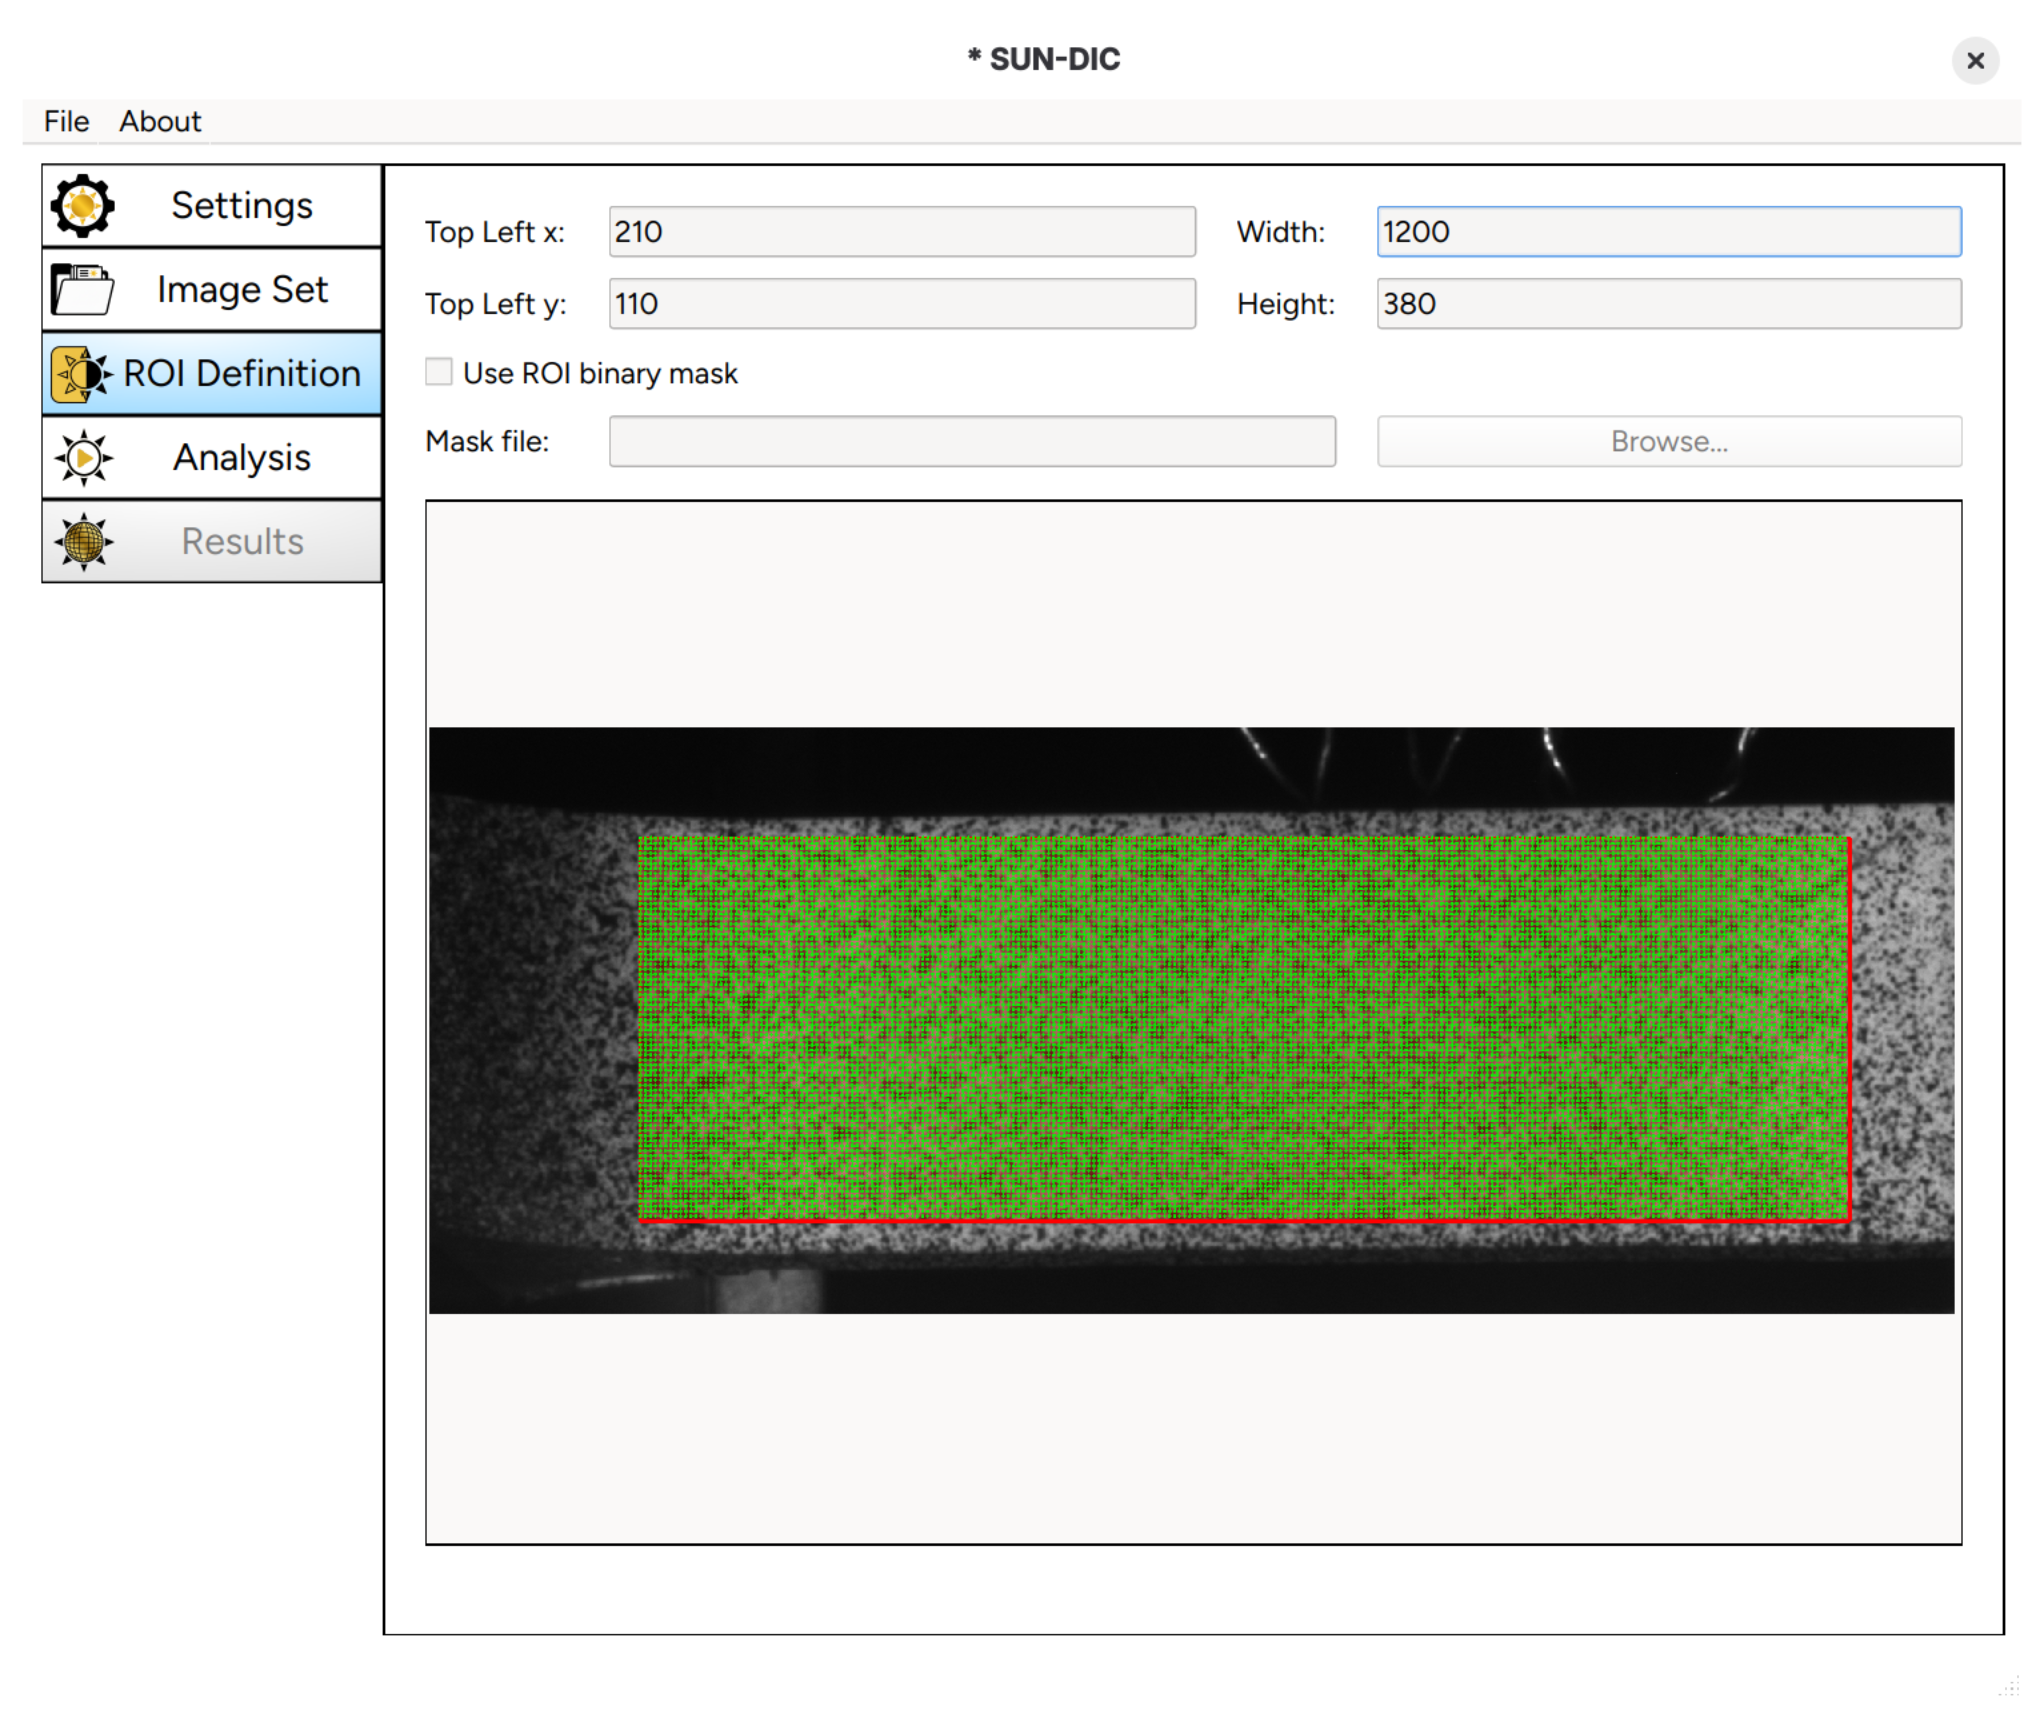
\includegraphics[width=0.85\textwidth]{../../screenshots/roi.png}
	\caption{ROI Definition Tab. Define the region of interest on the datum image.}
	\label{fig:gui_roi}
\end{figure}

\section{Analysis Tab}

The \codebf{Analysis} tab is used to perform the DIC analysis. Two runtime parameters can be configured in this tab:

\begin{itemize}
	\item \codebf{Debug Level} -- Controls verbosity of console output where 0 is no debug output, 1 corresponds to top-level output and 2 corresponds to per-iteration level output.  Note that debug output is limited when running the analysis in parallel.
	\item \codebf{CPU Count} -- The number of parallel worker processes to use during the analysis.
\end{itemize}

Click the \codebf{Start} button to begin the analysis. Live output is displayed in the output panel. The status indicator turns blue while running, green when complete, and red if the run is interrupted. Click the \codebf{Stop} button to abort execution.

Results are written to a binary \code{.sdic} file in the working directory. This file should not be saved inside the image directory, since all files in that directory are assumed to be image files during analysis.

\begin{figure}[htbp]
	\centering
	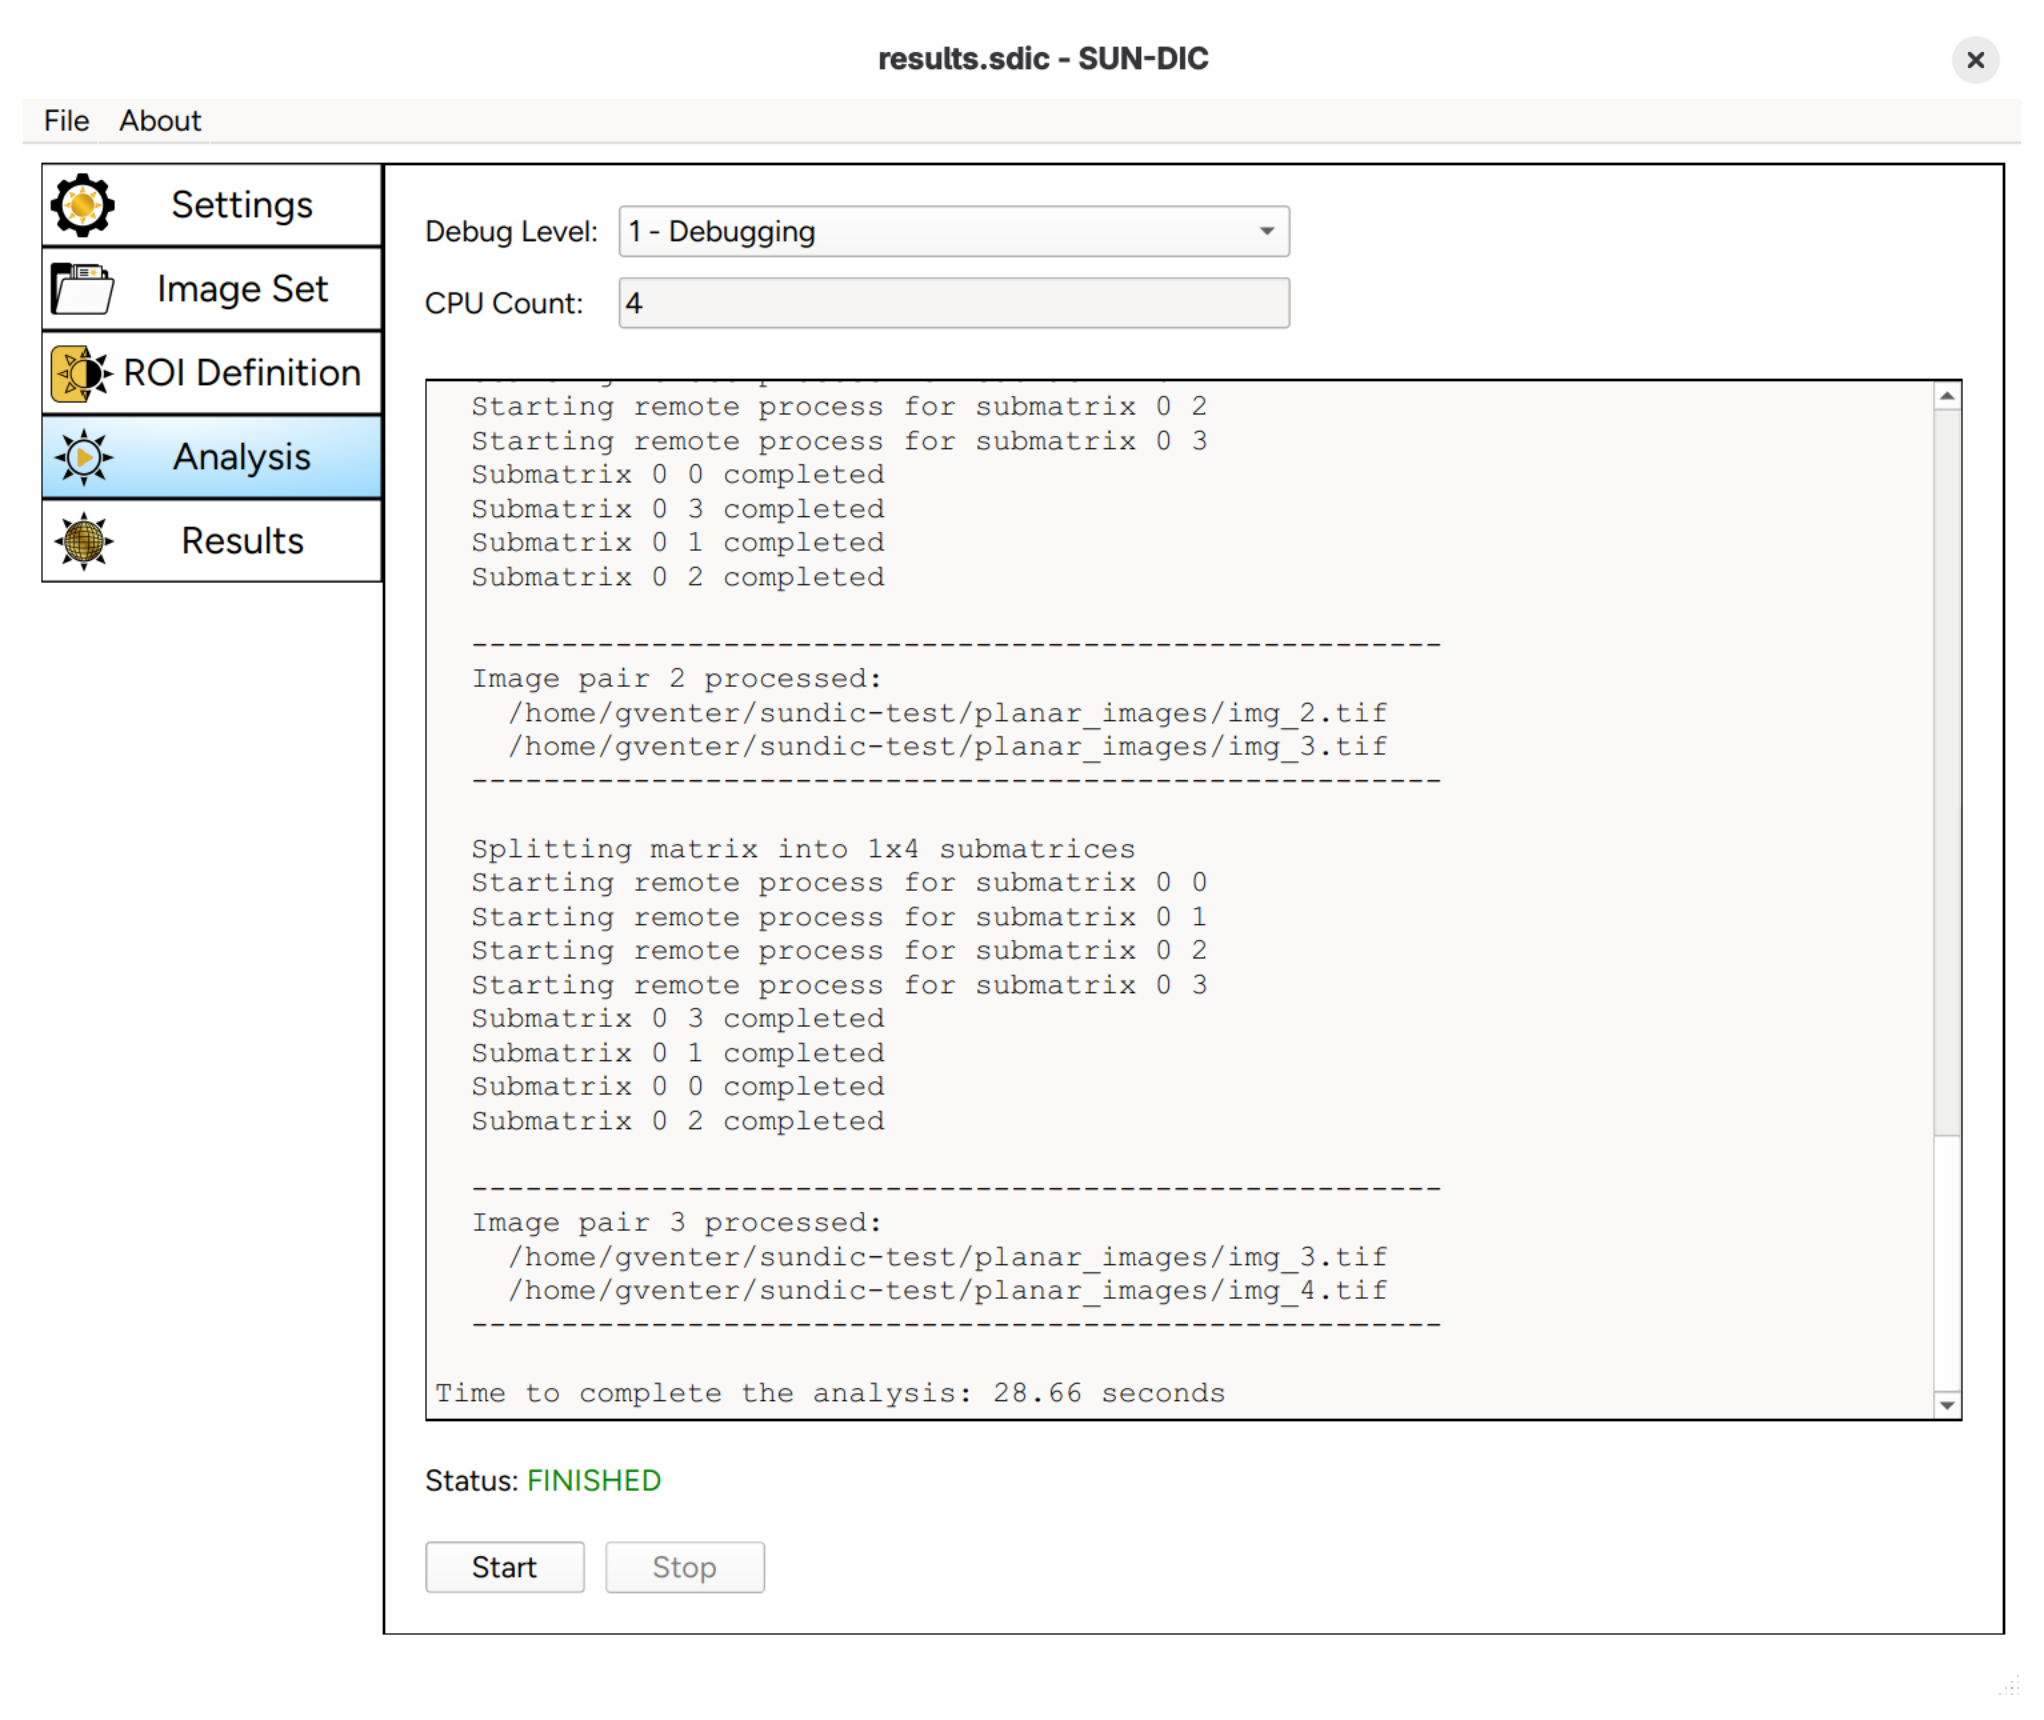
\includegraphics[width=0.85\textwidth]{../../screenshots/analyze.png}
	\caption{Analysis Tab. Run the DIC engine and monitor progress.}
	\label{fig:gui_analysis}
\end{figure}

\section{Results Tab}

The \codebf{Results} tab is used for post-processing the analysis results. The \codebf{Results} tab becomes active when there are results in the \code{.sdic} file, typically after the analysis is complete. Three view modes are available via the buttons at the top of the panel.

\begin{figure}[htbp]
	\centering
	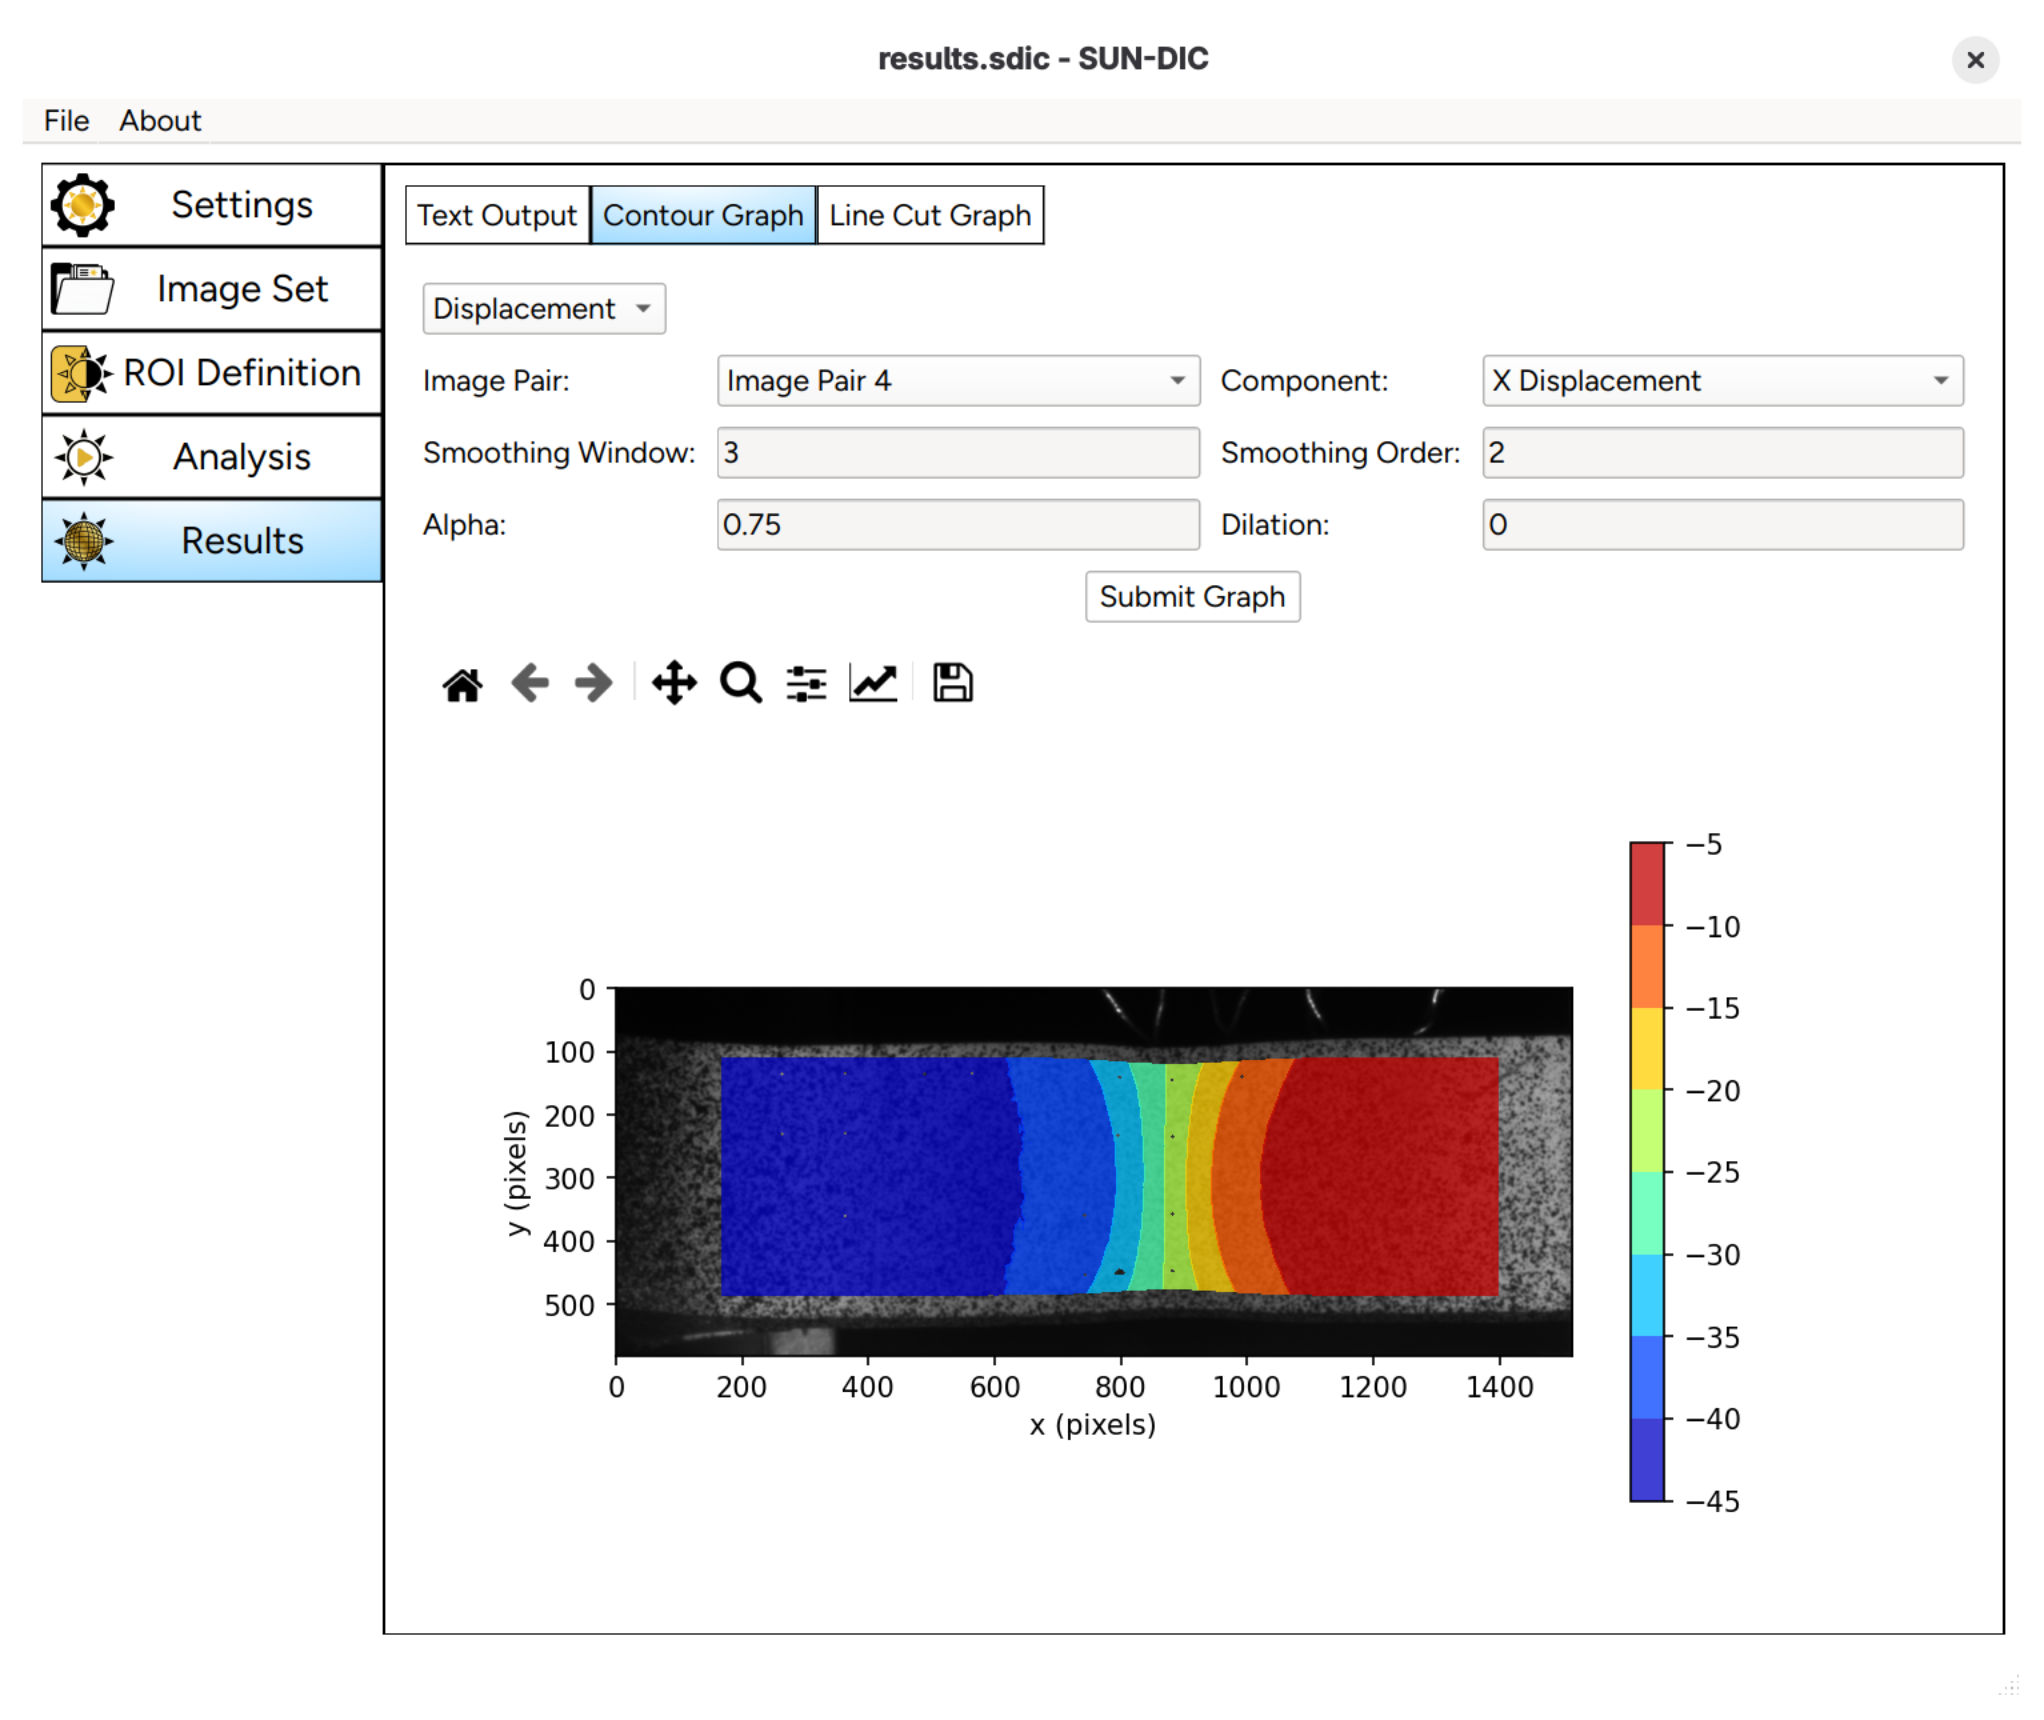
\includegraphics[width=0.85\textwidth]{../../screenshots/results.png}
	\caption{Results Tab. Contour plots, line cuts, and data export views.}
	\label{fig:gui_results}
\end{figure}

\newpage
\subsection{Contour Graph}

The \codebf{Contour Graph} panel is used to create contour plots of the computed field data over the specimen. This panel provides the following options:

\begin{itemize}
	\item \codebf{Results} -- Choose Displacement, Strain, or Correlation data to plot.
	\item \codebf{Image Pair} -- Select the image pair for post-processing.
	\item \codebf{Component} -- Select the field component: $u$ (X displacement), $v$ (Y displacement), displacement magnitude, $\varepsilon_x$, $\varepsilon_y$, $\varepsilon_{xy}$, or Von Mises strain $\varepsilon_\text{VM}$.
	\item \codebf{Smoothing Window / Order} -- Window size and polynomial order for Savitzky--Golay smoothing.
	\item \codebf{Alpha} -- Transparency of the contour overlay.
	\item \codebf{Dilation} -- Number of subsets to expand the exclusion mask, useful for edge cleaning.
\end{itemize}

Click the \textbf{Submit Graph} button to generate the plot.

\subsection{Line Cut Graph}

The \codebf{Line Cut Graph} panel is used to create two-dimensional line plots through the computed field data. A line-cut graph plots field values along one or more straight lines through the domain. This panel provides the following options:

\begin{itemize}
	\item \codebf{Results} -- Choose Displacement or Strain data to plot.
	\item \codebf{Image Pair} -- Select the image pair for post-processing.
	\item \codebf{Display Component} -- Select the field component: $u$ (X displacement), $v$ (Y displacement), displacement magnitude, $\varepsilon_x$, $\varepsilon_y$, $\varepsilon_{xy}$, or Von Mises strain $\varepsilon_\text{VM}$.
	\item \codebf{Cut Component} -- Axis along which cuts are taken (X or Y coordinate).
	\item \codebf{Cut Values} -- Comma-separated list of positions at which to make the cuts, e.g.\ \code{250, 300, 350}.
	\item \codebf{Smoothing Window / Order} -- Window size and polynomial order for Savitzky--Golay smoothing.
	\item \codebf{Dilation} -- Number of subsets to expand the exclusion mask, useful for edge cleaning.
	\item \codebf{Interpolate} -- Interpolate data onto a uniform grid before plotting. When this option is selected, the exact cut values are used. Otherwise, the nearest row or column of subset centres is used.
	\item \codebf{Grid Lines} -- Display grid lines on the graph.
\end{itemize}

Click the \textbf{Submit Graph} button to generate the plot.

\subsection{Text Output}

The \codebf{Text Output} panel is used to export the raw computed field data for external processing and provides the following options:

\begin{itemize}
	\item \codebf{Image Pair} -- Image pair to export.
	\item \codebf{Include Displacements / Strains} -- Select output fields to export.
	\item \codebf{Remove NaNs} -- Exclude failed or invalid subsets.
	\item \codebf{Smoothing Window / Order} -- Optional preprocessing before export. Uses a Savitzky--Golay filter to reduce noise in the exported data.
	\item \codebf{Dilation} -- Number of subsets to expand the exclusion mask, useful for edge cleaning.
\end{itemize}

Click the \textbf{Export Data} button to write the data to a \code{.csv} output file. The column structure matches the raw data format described in Section~\ref{sec:api}.

\section{Example Problem}

To run the example problem in the GUI, proceed as follows:

\begin{enumerate}
	\item Copy the example files to your working directory:
	
\begin{lstlisting}[language=bash]
copy-examples
\end{lstlisting}
	
	\textbf{This creates:}
	
	\begin{itemize}
		\item \code{test\_sundic.ipynb} -- Worked Python API example in Jupyter notebook format
		\item \code{settings.ini} -- Fully documented configuration file usable in both the GUI and API
		\item \code{planar\_images/} -- Sample TIFF image sequence for testing
	\end{itemize}
	
	\item Launch the GUI:
	
\begin{lstlisting}[language=bash]
sundic
\end{lstlisting}
	
	\item Import the \code{settings.ini} configuration via \textbf{File $\rightarrow$ Import Settings File}.
	
	\item Verify that settings, images, and ROI are correctly loaded. If the image files are not found, manually browse to the \code{planar\_images} folder.
	
	\item Run the analysis from the \textbf{Analysis} tab.
	
	\item Explore the results in the \textbf{Results} tab.
	
\end{enumerate}

You are encouraged to modify settings and rerun the analysis to explore different configurations and effects.
